\chapter{Overview of generative models in anomaly detection} \label{sec:chapter_survey}

\section{The Variational Autoencoder}

The Variational Autoencoder (VAE) model is a generative model based
on the classical autoencoder (AE). In its basic form, the architecture
is indeed very similar to that of an AE. The main difference is that
unlike in AE, where the encoding to latent space $\mathcal{Z}$ is
not constrained from taking any shape or form as far as the learning
objective is minimized, in VAE a desired shape of the encoding is
explicitly prescribed in the form of a prior distribution $p(z)$.
If the network is trained properly and the encoder is not far from
the desirable shape, we can feed samples from $p(z)$ to the decoder
and expect to obtain random samples in the $\mathcal{X}$ space that
will however resemble those from the training dataset. This is the
simple explanation of how VAE works --- we will dwell into the details
in the following text.

The VAE has enjoyed a great success in a number of fields since its
introduction in\,\cite{kingma2013vae}. Its has been mainly used
for generation of artificial images such as faces\,\cite{rezende2014stochastic}
but also for other tasks such as semi--supervised learning\,\cite{kingma2014semi},
segmentation\,\cite{sohn2015learning}, static image forecasting\,\cite{walker2016uncertain}
and of course for anomaly detection\,\cite{an2015variational,xu2018unsupervised,solch2016variational}.
Since its popularity, a multitude of approaches enhancing the original
VAE has been published, approaching the paradigm from different angles,
with some of the more prominent examples published in\,\cite{higgins2017beta,zhao2017infovae,tolstikhin2017wasserstein,makhzani2015adversarial,pu2017adversarial}.
In the following text, we will go through the basic theory and its
implications for the basic VAE and then through some of the extensions.
Also, we will try to assess the suitability of the presented models
for anomaly detection.

\subsection{Probabilistic foundations}

We will begin by defining the Variational Autoencoder from a probabilistic
perspective. In fact, the connection with autoencoders will become
apparent only after all the derivations have been carried out. Let
us assume that there is a dataset $X=\{x_{i}\}_{i=1}^{N}$ consisting
of i.i.d samples. We want to obtain a tractable estimate of the true
data distribution $p(x)$ in order to be able to sample from it. For
that purpose, suppose that there is a hidden random process that generates
the data and which involves a latent variable $z$. Then, we can redirect
the sampling from the data space $\mathcal{X}$ to the latent space
$\mathcal{Z}$, in which it might be easier. Specifically, we want
to sample from the latent distribution specified by density $p(z)$,
then pass this to the generative model distribution $p_{\theta}(x|z)$
with parameters $\theta$ and obtain a sample $x$ that will be very
similar to the samples coming from $p(x)$. In other words, we want
to maximize the probability of each sample obtained through the generative
process
\begin{equation}
p_{\theta}(x)=\int_{\mathcal{Z}}p_{\theta}(x|z)p(z)dz.\label{eq:x_likelihood}
\end{equation}
Unfortunately, there are several issues with this. Firstly, we do
not know the optimal value of parameters $\theta$. Secondly, the
integral\,(\ref{eq:x_likelihood}) is usually intractable, e.g. in
the case where $p_{\theta}(x|z)$ is represented by a neural network.
Finally, we want to avoid expensive sampling methods such as Monte
Carlo Expectation Maximization which might offer a solution. We will
use a sampling procedure in the end, but we only want to pass such
samples $z$ to the generative model that will already be very likely
under $p_{\theta}(x|z)$. To this end, we introduce a recognition
model $q_{\phi}(z|x)$ which is an approximation of the true intractable
posterior $p(z|x)$ parametrized by $\phi$.

\subsection{The ELBO objective}

Now, we would like to relate all the introduced probability distributions
together in way that would enable us to optimize the recognition and
the generative model in respect to $\phi,\theta$. Continuing from\,(\ref{eq:x_likelihood}),
\begin{equation}
\ln p_{\theta}(x)=\mathbb{E}_{q_{\phi}(z|x)}\left[\ln p_{\theta}(x)\right]=\mathbb{E}_{q_{\phi}(z|x)}\left[\ln p_{\theta}(x|z)+\ln p(z)-\ln p(z|x)\right],
\end{equation}
where we have used the Bayes' rule and the fact that $p_{\theta}(x)$
does not depend on $z$. Now we recall the definition of the KL divergence\,(\ref{eq:kld})
\begin{eqnarray}
\ln p_{\theta}(x)-D_{\text{KL}}\left(q_{\phi}(z|x)||p(z|x)\right) & = & \mathbb{E}_{q_{\phi}(z|x)}\left[\ln p_{\theta}(x|z)+\ln p(z)-\ln q_{\phi}(z|x)\right]\label{eq:elbo1}\\
 & = & \mathbb{E}_{q_{\phi}(z|x)}\left[\ln p_{\theta}(x|z)\right]-D_{\text{KL}}\left(q_{\phi}(z|x)||p(z)\right)\label{eq:elbo2}\\
 & = & \mathcal{L}(x,\phi,\theta)\label{eq:elbo3}
\end{eqnarray}
Now, we have a variational lower bound $\mathcal{L}(x,\phi,\theta)$
(sometimes called ELBO -- evidence lower boundary) through which
we can optimize the marginal likelihood $p_{\theta}(x)$. This is
due to the fact that the analytically unsolvable term $D_{\text{KL}}\left(q_{\phi}(z|x)||p(z|x)\right)$
is always nonnegative, thus by maximization of $\mathcal{L}(x,\phi,\theta)$
we also maximize $p_{\theta}(x)$.

Let us dissect the individual parts of the above equation. By looking
at the individual parts of Eq.\,(\ref{eq:elbo2}), we can see that
by maximizing the ELBO, we simultaneously maximize the likelihood
$p_{\theta}(x|z)$ and minimize the distance between $q_{\phi}(z|x)$
and $p(z)$. While looking at the left--hand side of (\ref{eq:elbo1})
we can see that in the same process, the marginal likelihood $p_{\theta}(x)$
is maximized and the error term $D_{\text{KL}}\left(q_{\phi}(z|x)||p(z|x)\right)$
is minimized, forcing the shape of $q_{\phi}(z|x)$ to the true posterior.
Also, from\,(\ref{eq:elbo2}) it is now apparent why this model is
called an autoencoder. We pass $x$ to the recognition model (encoder),
produce latent $z$ and pass this back to the generative model (decoder)
to obtain a reconstructed sample.
\begin{figure}
\centering{}\begin{tikzpicture}
  \node[const]                               (x) {$\vc{x}$};
  \node[const, right = 0.4cm of x]           (xin) {};
  % encoder in
  \node[latent, right = 0.4cm of x, yshift = 0.825cm] (E11) {};
  \node[latent, right = 0.4cm of x, yshift = 0.275cm] (E12) {};
  \node[latent, right = 0.4cm of x, yshift = -0.275cm] (E13) {};
  \node[latent, right = 0.4cm of x, yshift = -0.825cm] (E14) {};
  % encoder hidden
  \node[latent, right = 1.6cm of x, yshift = 0.55cm] (E21) {};
  \node[latent, right = 1.6cm of x, yshift = 0cm] (E22) {};
  \node[latent, right = 1.6cm of x, yshift = -0.55cm] (E23) {};
  % encoder out
  \node[latent, right = 2.8cm of x, yshift = 0.9cm] (E31) {};
  \node[latent, right = 2.8cm of x, yshift = 0.35cm] (E32) {};
  \node[latent, right = 2.8cm of x, yshift = -0.35cm] (E33) {};
  \node[latent, right = 2.8cm of x, yshift = -0.9cm] (E34) {};
  % encoder tag
  \node[const, right = 1.6cm of x, yshift = 1.4cm] (ED) {$q_{\vc{\phi}}(\vc{z}|\vc{x})$};
  % code
  \node[const, right = 3.8cm of x, yshift = 0.575cm]           (mu) {$\vc{\mu}_{\vc{\phi}}$};
  \node[const, right = 3.8cm of x, yshift = -0.575cm]           (sigma) {$\vc{\sigma}^2_{\vc{\phi}}$};
  \node[const, right = -1.0cm of mu]           (muout) {};       
  \node[const, right = -1.0cm of sigma]           (sigmaout) {};       
  \node[const, right = 4.8cm of x, yshift=-0.1cm]           (z) {$z=\mu_{\vc{\phi}}+\sigma_{\vc{\phi}} \odot \varepsilon$};
  \node[const, right = -2.7cm of z]           (zout) {};
  \node[const, right = 4.95cm of x, yshift = 0.9cm]         (epsilon) {$\varepsilon \sim \mathcal{N}(0,\vc{I})$};
  \node[const, right = 5.9cm of x, yshift = 0.2cm]         (epsilonin) {};
  \node[const, right = 0.5cm of z]           (zin) {};
  % decoder in
  \node[latent, right = 0.6cm of z, yshift = 0.275cm] (D11) {};
  \node[latent, right = 0.6cm of z, yshift = -0.275cm] (D12) {};
  % decoder hidden
  \node[latent, right = 1.8cm of z, yshift = 0.55cm] (D21) {};
  \node[latent, right = 1.8cm of z, yshift = 0cm] (D22) {};
  \node[latent, right = 1.8cm of z, yshift = -0.55cm] (D23) {};
  % decoder out
  \node[latent, right = 3cm of z, yshift = 0.825cm] (D31) {};
  \node[latent, right = 3cm of z, yshift = 0.275cm] (D32) {};
  \node[latent, right = 3cm of z, yshift = -0.275cm] (D33) {};
  \node[latent, right = 3cm of z, yshift = -0.825cm] (D34) {};
  % xhat
  \node[const, right = 4cm of z]           (xhat) {$\vc{x}'$};
  \node[const, right = -0.8cm of xhat]       (xhatout) {};    
  % decoder tag
  \node[const, right = 1.6cm of z, yshift = 1.4cm] (DD) {$p_{\vc{\theta}}(\vc{x}|\vc{z})$};   
  
  % edges
  \nedge {x} {xin}
  % encoder 
  \nedge {E11, E12, E13, E14} {E21, E22, E23}
  \nedge {E21, E22, E23} {E31, E32, E33, E34}
  % latent
  \nedge {muout} {mu}
  \nedge {sigmaout} {sigma}
  \nedge {mu,sigma} {zout}
  \nedge {z} {zin}
  \nedge {epsilon} {epsilonin}
  % decoder
  \nedge {D11, D12} {D21, D22, D23}
  \nedge {D21, D22, D23} {D31, D32, D33, D34} 
  %xhat
  \nedge {xhatout} {xhat}
\end{tikzpicture}
\caption{A schematic of a Variational Autoencoder consisting of fully connected
layers with the encoder $q_{\phi}(z|x)$ parametrizing a normal distribution.
A mean $\mu$ and variance vector $\sigma^{2}$ are extracted from
the last layer of the encoder. They are used to sample a code $z$
from the corresponding normal distribution and then passed to the
decoder $p_{\theta}(x|z)$ to produce the reconstruction $\tilde{x}.$}
\label{fig:vae}
\end{figure}


\subsection{The reparametrization trick}

Often, the KL divergence in\,(\ref{eq:elbo2}) can be computed analytically
based on our choice of $p(z)$. Furthermore, to optimize the ELBO,
we need to sample from $q_{\phi}(z|x)$. A usual choice of the prior
is $p(z)=\mathcal{N}(z|0,I)$, but any continuous distribution is
theoretically viable. In tandem with this, the shape of the recognition
distribution should be the same, i.e. $q_{\phi}(z|x)=\mathcal{N}(z|\mu_{\phi}(x),\Sigma_{\phi}(x))$.
This is however problematic for training through backpropagation,
because sampling is not a differentiable operation. Therefore, to
be able to optimize $\phi$, a reparametrization trick must be used.
Instead of drawing samples $z\sim\mathcal{N}(z|\mu_{\phi}(x),\Sigma_{\phi}(x))$,
we first take a sample from noise distribution $\varepsilon\sim p(\varepsilon)=\mathcal{N}(0,1)$
and then compute $z=\mu_{\phi}(x)+\Sigma_{\phi}^{1/2}(x)\varepsilon$.
This changes the ELBO to
\begin{equation}
\mathcal{L}(x,\phi,\theta)=\mathbb{E}_{\varepsilon\sim\mathcal{N}(0,I)}\left[\ln p_{\theta}(x|z=\mu_{\phi}(x)+\Sigma_{\phi}^{1/2}(x)\varepsilon)\right]-D_{\text{KL}}\left(q_{\phi}(z|x)||p(z)\right).\label{eq:vae_loss}
\end{equation}
Note that in practice, where encoder $q_{\phi}(x|z)$ is represented
by a neural network, the distribution parameters are extracted from
its last layer. While linear activation is used for $\mu_{\phi}(x)$,
softplus is usually used for $\Sigma_{\phi}(x)$.

\subsection{Vanilla VAE\label{sec:vae_vanilla}}

In this section we will describe the single most common VAE architecture
with the recognition model being $q_{\phi}(z|x)=\mathcal{N}(z|\mu_{\phi}(x),\text{diag}(\sigma_{\phi}^{2}(x))),\mu_{\phi}(x),\sigma_{\phi}^{2}(x)\in\mathbb{R}^{d}$.
This, together with the fact that $p(z)=\mathcal{N}(z|0,I)$ makes
the computation of the KL divergence in\,(\ref{eq:elbo2}) analytically
tractable, see\,(\ref{eq:kl_standard}). The ELBO for a single datapoint
then takes the form
\begin{eqnarray*}
\mathcal{L}(x,\phi,\theta;\varepsilon) & = & \frac{1}{M}\sum_{m=1}^{M}\ln p_{\theta}(x|z^{m}(\varepsilon))+\frac{1}{2}\sum_{i=1}^{d}\left(1-\left(\sigma_{\phi}^{2}(x)\right)_{i}+\ln\left(\sigma_{\phi}^{2}(x)\right)_{i}-\left(\mu_{\phi}^{2}(x)\right)_{i}\right)
\end{eqnarray*}
\begin{equation}
\text{where }z^{m}(\epsilon)=\mu_{\phi}(x)+\sigma_{\phi}(x)\odot\varepsilon,\varepsilon\sim\mathcal{N}(0,I).\label{eq:vae_elbo1}
\end{equation}
The expectation for the marginal likelihood is replaced with a mean
over $M$ samples of $\varepsilon\sim p(\varepsilon)$ and $\odot$
denotes an element--wise product. Note that $M=1$ is usually sufficient
given that the model is trained with high enough batchsize. Now, $p_{\theta}(x|z)$
can take the form of any suitable distribution (e.g. normal or Bernoulli).
The most common choice is the case of a normal isotropic generative
model, that is $p_{\theta}(x|z)=\mathcal{N}(x|\mu_{\theta}(z),\Sigma_{\theta}(z))=\mathcal{N}(x|\mu_{\theta}(z),\sigma I),\sigma\in\mathbb{R}$.
Then, the optimization objective becomes
\begin{equation}
\mathcal{L_{\text{VAE}}}(x,\phi,\theta;\varepsilon)=-\frac{1}{\sigma M}\sum_{m=1}^{M}||x-\mu_{\theta}(z^{m}(\varepsilon))||_{2}^{2}+\frac{1}{2}\sum_{i=1}^{d}\left(1-\left(\sigma_{\phi}^{2}(x)\right)_{i}+\ln\left(\sigma_{\phi}^{2}(x)\right)_{i}-\left(\mu_{\phi}^{2}(x)\right)_{i}\right)\label{eq:vae_elbo2}
\end{equation}
with $z^{m}(\varepsilon)$ sampled in the same way as in\,(\ref{eq:vae_elbo1}).
Finally, this objective can be optimized via stochastic gradient descent\,\cite{bottou2010large}.

See Fig.\,\ref{fig:vae} for a schematic example of a VAE architecture
that uses the loss function\,(\ref{eq:vae_elbo2}). The training
procedure of a VAE is described in Alg.\,\ref{alg:vae_train}. Note
that instead of setting a fixed variance parameter $\sigma$ in the
decoder, one can optimize and extract it instead from the last layer
of the decoder, either as a scalar $\Sigma_{\theta}(z)=\sigma_{\theta}(z)I,\sigma(z)\in\mathbb{R}$
or even full diagonal of the covariance $\Sigma_{\theta}(z)=\text{diag}\left(\sigma_{\theta}(z)\right)I,\sigma(z)\in\mathbb{R}^{n}$
where $n$ is the dimensionality of input space $\mathcal{X}$. See
the discussion in Fig.\,\ref{fig:betavae} for details.

\begin{algorithm}
\begin{algorithmic}[1]
\Require{A VAE model with encoder $q_{\vc{\phi}}(\vc{z}|\vc{x})$ and decoder $p_{\vc{\theta}}(\vc{x}|\vc{z})$, training set $X=\lbrace \vc{x}_1, \vc{x}_2, \ldots, \vc{x}_n \rbrace \subset \mathcal{X}$, maximum number of iterations $I\in\mathbb{N}$, batchsize $B \in \mathbb{N}$.}
\State $\vc{\phi},\vc{\theta} \gets $ Initialize parameters
\State{$i \gets $ Iteration counter}
\While{$i<I$ or $\vc{\phi},\vc{\theta}$ are not converged}
	\State{$X_B \gets$ A random batch of $B$ samples from $X$}
	\State$l \gets \frac{1}{B}\sum_{j=1}^L \mathcal{L}_\text{VAE}(\vc{x}_j,\vc{\phi},\vc{\theta}), \vc{x}_j \in X_B$
	\State$\vc{\phi} \stackrel{+}\gets - \nabla_{\vc{\phi}}l $ update of encoder weights
	\State$\vc{\theta} \stackrel{+}\gets - \nabla_{\vc{\theta}}l $ update of decoder weights
	\State{$i \gets i+1$}
\EndWhile
\State{\textbf{return} encoder $q_{\vc{\phi}}(\vc{z}|\vc{x})$, decoder $p_{\vc{\theta}}(\vc{x}|\vc{z})$}
\end{algorithmic}\caption{Variational Autoencoder training procedure.}
\label{alg:vae_train}
\end{algorithm}

Now that a VAE model is trained, we can finally use it to generate
realistic samples. Because we have pushed the encoding distribution
to be close to the prior while maximizing the marginal probability
of the encoding to produce a reasonable reconstruction through the
decoder, we can expect the converged decoder to be able to transform
samples $z\sim\mathcal{N}(0,1)$ to the $\mathcal{X}$ space in such
a manner that they will be very close to the samples from the training
dataset. This is also a place to note why we are using neural network
representation of $q_{\phi}(z|x)$ and $p_{\theta}(x|z)$. Since NNs
have be proven to be universal function approximators, we know that
given enough capacity, data and training time, the decoder can learn
a mapping from $\mathcal{N}(0,1)$ to arbitrary function.

What is of a greater interest to us from the anomaly detection perspective
is reconstructing a sample using the trained VAE. This is done through
the same process the VAE is trained, thus by reconstruction of $x$
we understand $\hat{x}$ such that
\begin{equation}
\hat{x}\sim\mathcal{N}(x|\mu_{\theta}(z),\Sigma_{\theta}(z)),z\sim q_{\phi}(z|x).
\end{equation}
We simply pass $x$ to the encoder $q_{\phi}(z|x)$, obtain the parameters,
sample from the noise distribution and pass the resulting $z$ to
the decoder $p_{\theta}(x|z)$ to obtain the generative distribution
from which we can readily sample.

Looking at the objective\,(\ref{eq:vae_elbo2}) we can see the connection
with an ordinary autoencoder. The objective can be decomposed into
a reconstruction term and a regularization term on the latent space.
The one advantage of a VAE over AE is that provides a distribution
both in the latent and sample space that can be readily sampled from,
while the autoencoder is completely deterministic. This, coupled with
the regularization term, enables the VAE to generalize better.

It has been shown in\,\cite{doersch2016tutorial} that scaling of
the VAE loss\,(\ref{eq:vae_elbo2}) with respect to the variance
estimated by the encoder does not make much sense. It is however possible
to scale the contribution of the two losses to the total loss, as
was done in\,\cite{higgins2017beta}, such that
\begin{equation}
\mathcal{L}(x,\phi,\theta,\beta)=\mathbb{E}_{q_{\phi}(z|x)}\left[\ln p_{\theta}(x|z)\right]-\beta D_{\text{KL}}\left(q_{\phi}(z|x)||p(z)\right),\beta>0.\label{eq:betavae}
\end{equation}
Varying the value of $\beta$ puts a different emphasis on how much
should the latent space be regularized. Higher values of $\beta$
supposedly lead to better representation power, however in some of
our experiments we have used $\beta<1$ in order to pronounce the
importance of the reconstruction error. Again, the discussion under
Fig.~\ref{fig:betavae} contains some details on this.

\begin{figure}
\centering
    \begin{subfigure}[b]{0.45\textwidth}
        \centering
        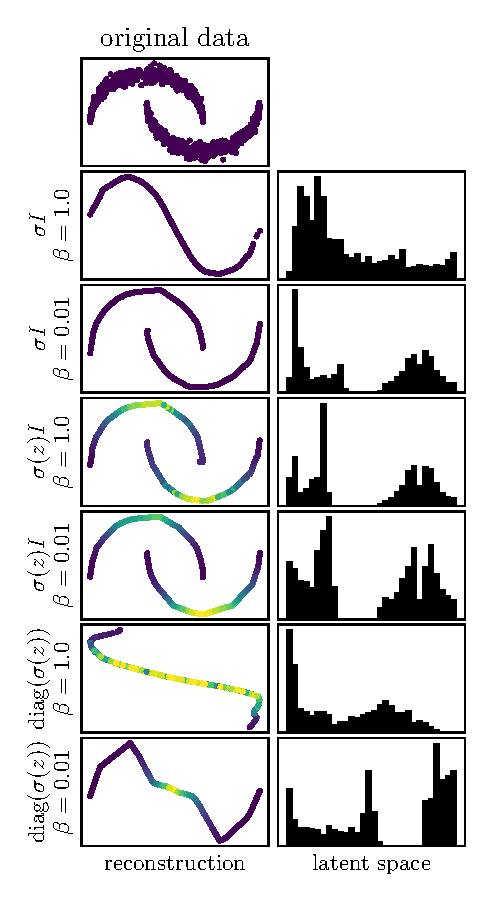
\includegraphics[scale=0.9]{data/chapter_survey/vae_two_moons_z1_colored}
        \caption{$\text{dim}(\mathcal{Z})=1$}
    \end{subfigure}
    \begin{subfigure}[b]{0.45\textwidth}
        \centering
        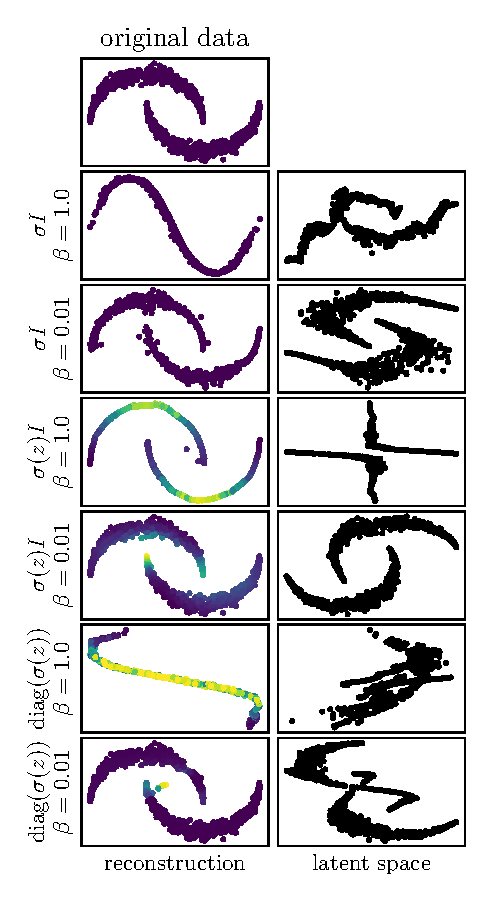
\includegraphics[scale=0.9]{data/chapter_survey/vae_two_moons_z2_colored}
        \caption{$\text{dim}(\mathcal{Z})=2$}
    \end{subfigure}
\caption{An overview of VAE behaviour with respect to the scaling parameter
$\beta$ of the objective\,(\ref{eq:betavae}) and to the way the
covariance of the generative model $p_{\theta}(x|z)=\mathcal{N}(x|\mu_{\theta}(z),\Sigma_{\theta}(z))$
is estimated. The VAE model was trained on the two--moons data, plotted
in the plots at the very top. Variants with 1D (a) and 2D (b) latent
spaces are compared, means of the generative model $\mu_{\theta}(z)$
are plotted on the left and the latent representations on the right.
Clearly, smaller values of $\beta$ lead to better sample reconstruction.
Also, lower preference of the KL divergence objective seems to lead
to better separation in the latent space. This is understandable,
since the prior $p(z)=\mathcal{N}(0,1)$ is unimodal. The covariance
is given by a fixed scalar ($\Sigma=\sigma I,\sigma=1$), by a scalar
estimated from the data ($\Sigma=\sigma(z)I$), or the full diagonal
of the covariance matrix is estimated ($\Sigma=\text{diag}(\sigma(z))$).
The magnitude of the estimated variance in the two latter cases is
denoted by color, where brighter color corresponds to a higher value.
It is interesting that the second case ($\Sigma=\sigma(z)I$) seems
to alleviate the reconstruction difficulties with higher $\beta$,
while the estimation of the full covariance diagonal does not exhibit
such property. Also, the third case seems to ``exploit'' the estimation
of variance -- instead of pushing and optimizing the mean, it can
instead simply put higher variance in the direction in which the reconstruction
is worse and still incur only a small loss. Due to this behaviour,
the second case seems to be the most robust and stable way of estimation
of the reconstruction variance. Not surprisingly, the 2D case provides
better reconstructions since it was provided with one more dimension
to encode data to.}
\label{fig:betavae}
\end{figure}

\begin{figure}
\centering{}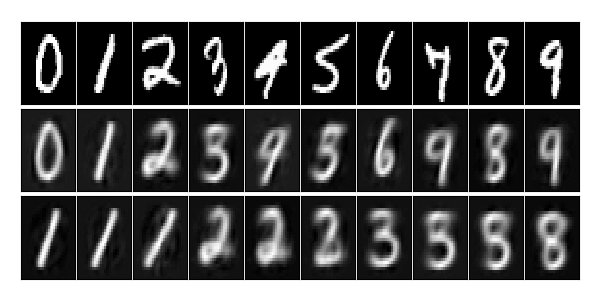
\includegraphics[scale=0.8]{data/chapter_survey/mnist_reconstruction_generation}\caption{Example of a VAE trained on the MNIST dataset -- ground truth examples
are in the top row, reconstructed samples (means of $p_{\theta}(x|z)$)
are in the middle row, artificially generated digits are in the bottom
row. The reconstructions are blurry, which is a typical VAE behaviour.
Also, the reconstruction is imperfect for digits which are resemble
each other, such as 9, 4 and 7 or 3 and 8. The artificial digits were
created by linearly interpolating between two coordinates in the latent
space and using this as an input to the decoder. The VAE then presents
a smooth interpolation between digits 1 and 8.}
\label{fig:mnist_reconstruction}
\end{figure}
 
\begin{figure}
\begin{centering}
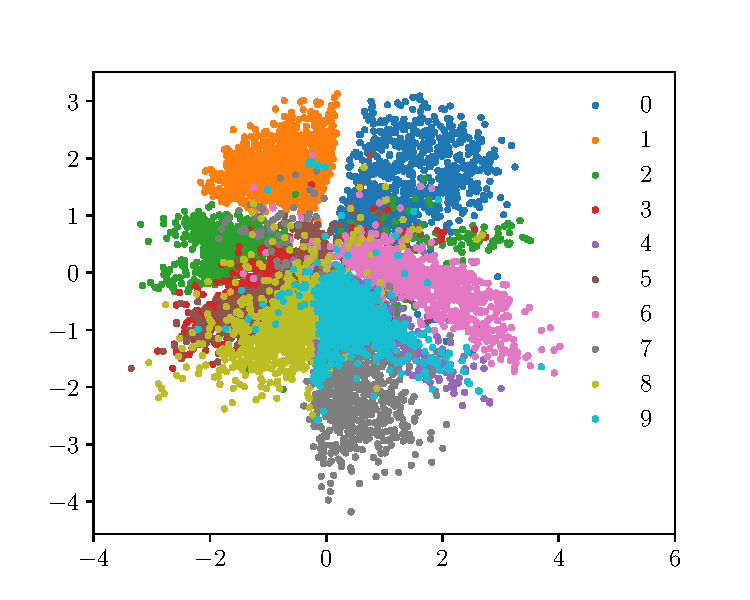
\includegraphics[scale=0.8]{data/chapter_survey/mnist_latent}
\par\end{centering}
\caption{The latent space of the MNIST dataset produced by a VAE. Note the
overlapping of some digit encodings, e.g. 7 and 9.}
\label{fig:mnist_latent}
\end{figure}

We include some experiments with the MNIST hand--written digits dataset,
which can be found in almost every VAE publication, see Fig.\,\ref{fig:mnist_reconstruction}
and \ref{fig:mnist_latent}, that demonstrate the way a VAE encodes,
reconstructs and generates new samples.

\subsection{VAE in anomaly detection}

An easy way to assess the probability of a sample coming from the
data distribution would be computing 
\begin{equation}
p_{\theta}(x)=\mathbb{E}_{p(z)}\left[\ln p_{\theta}(x|z)\right]
\end{equation}
by sampling directly from the prior. Although theoretically well--justified,
it has been shown that this does not work well enough in practice\,\cite{xu2018unsupervised}.
Instead, the reconstruction probability can be used as an anomaly
score function
\begin{equation}
f_{\text{VAE}}(x)=-\frac{1}{M}\sum_{m=1}^{M}\ln p_{\theta}(x|z^{m}(\varepsilon))\approx-\mathbb{E}_{q_{\phi}(z|x)}\left[\ln p_{\theta}(x|z)\right].\label{eq:vae_score}
\end{equation}
which was done in one of the first application of VAE in anomaly detection
in\,\cite{an2015variational}. The negative sign is used because
of the convention of higher score belonging to an anomaly. Note that
for a Gaussian decoder, equation\,(\ref{eq:vae_score}) is very similar
to the reconstruction error of a standard autoencoder with the difference
that the reconstruction probability is computed from several samples
of the noise distribution. Because there is sampling in the latent
space, this anomaly score can process the variability of the input
space in an improved way. We suppose that an anomalous sample that
the VAE has not been trained with will have a lower probability of
being correctly reconstructed, thus producing a higher anomaly score.
The authors of\,\cite{an2015variational} successfully compare VAE
with AE and PCA on several anomaly datasets while claiming that the
generative property of VAE can be used for causal analysis on the
detected anomalies.

The reason for using the reconstruction probability of a VAE instead
of a reconstruction error of AE is the improved generalization that
was described in the previous section. It is discussed in\,\cite{dai2017hidden}
that a VAE model is equivalent to a non--linear robust PCA model
and is proficient at dismissing sparse outliers. The authors also
make note of the fact that VAE is very efficient in pruning of unnecessary
latent dimensions in case when the real latent structure has lower
dimension than the chosen VAE latent space. However, sometimes\,\cite{pereira2018unsupervised}
the reconstruction error of the VAE is used, which is defined as
\begin{equation}
f_{\text{VAEr}}(x)=-\frac{1}{M}\sum_{m=1}^{M}||x-\mathbb{E}\left[p_{\theta}(x|z^{m}(\varepsilon)\right]||_{2}^{2},
\end{equation}
where only the mean of the generative distribution is compared to
the original sample $x$.

Another way of using VAE and other autoencoding models for anomaly
detection is to employ their ability to produce a low--dimensional
representation of high--dimensional data that preserves the important
relations between individual datapoints. Then, an anomaly detection
model (be it a generative or a classical one) can be trained on the
data encoded in the latent space. This two stage approach is especially
useful when the problem is in the image domain and some kind of vectorization
has to be used anyway. Also it enables the combination of countless
different approaches. Usage of this technique will be demonstrated
in one of the next chapters. It is also used in\,\cite{dai2019diagnosing},
where both stages are a VAE and the second stage has the same input
and latent space dimensionality (therefore it does not compress data
at all). Although this paper does not present an application in anomaly
detection, it shows an improvement in learning of the latent space
prior. 

In\,\cite{xu2018unsupervised} the authors present a so-called DonutVAE
with an enhanced loss function to detect anomalies in times series
data. The architecture is similar to that of a vanilla VAE, but the
loss becomes
\begin{equation}
\mathcal{L}_{\text{DVAE}}(x,\phi,\theta)=\mathbb{E}_{q_{\phi}(z|x)}\left[\beta\ln p(z)-\ln q_{\phi}(z|x)+\sum_{t=i}^{T}\alpha_{t}\ln p_{\theta}(x|z)\right],\label{eq:donutvae}
\end{equation}
where $x=\{x_{t}\}_{t=1}^{T}$ is a sliding window of the last $T$
observations. Also, $\alpha_{t}=0$ if $x_{t}$ is anomalous or missing
and $\alpha_{t}=1$ otherwise and $\beta=\sum_{t=1}^{T}\alpha_{t}/T$.
The authors then show that usage of this loss function improves overall
results. This however has a caveat -- known anomalous samples must
be available, otherwise the loss\,(\ref{eq:donutvae}) is the same
as\,(\ref{eq:elbo2}). Furthermore, the authors claim that using
reconstruction probability\,(\ref{eq:vae_score}) can be seen as
a weighted kernel density estimate.

The authors of\,\cite{zong2018deep} couple an ordinary autoencoder
with a Gaussian mixture model (GMM) represented by a neural network.
The AE reduces the problem dimension to help overcome the curse of
dimensionality, while the GMM model serves as a density estimate in
the latent space. The novelty of the method is in two facts. Firstly,
instead of training parameters of both models separately, they are
learnt jointly which improves the performance of the model. Secondly,
the input of the GMM model is not only the latent representation,
but also the reconstruction error of the sample. The loss is 
\begin{eqnarray}
\mathcal{L}_{\text{DAGMM}}(x,\phi,\theta,\omega) & = & ||x-d_{\theta}(e_{\phi}(x))||_{2}^{2}+\lambda_{1}E_{\omega}(z)+\lambda_{2}P(\hat{\Sigma)}\\
z & = & \left[e_{\phi}(x),||x-d_{\theta}(z)||_{2}^{2}\right]^{T}\\
E_{\omega}(z) & = & -\ln\left(\sum_{i=1}^{d}\pi_{\omega,i}\frac{\exp\left(-\frac{1}{2}(z-\mu_{\omega,i})^{T}\Sigma_{i}^{-1}(z-\mu_{\omega,i})\right)}{\sqrt{|2\pi\Sigma_{\omega,i}|}}\right)
\end{eqnarray}
where we recognize the reconstruction error of the AE, the energy
term $E_{\omega}(z)$ of the GMM model and a penalization $P(\Sigma)$
that prevents the covariance matrices in the GMM model to become singular,
$\lambda_{1},\lambda_{2}>0$ are scaling parameters. Parameters $\left\{ \pi_{\omega,i},\mu_{\omega,i},\Sigma_{\omega,i}\right\} _{i=1}^{d}$
are the parameters of the GMM model estimated by a neural network
with weights $\omega$. The sample energy is used as anomaly score.
Although this model is not based on VAE, we can view the energy term
as being similar to the KL divergence term in the VAE loss as it also
imposes some kind of structure in the latent space.

A VAE model couple with an LSTM recurrent neural network with attention
mechanism is used in\,\cite{pereira2018unsupervised} for detecting
anomalies in time series. They operate in the semisupervised setting,
where only labeled normal samples are used for training. Although
the authors share some interesting insights, e.g. that the VAE is
able to capture the temporal structure in the data, they do not offer
a thorough comparison with other methods.

\section{GAN--based models}

A different sort of generative deep model has been successful recently
-- the Generative Adversarial Network (GAN)\,\cite{goodfellow2014gan}.
It is based on a different perspective than the VAE model. Generally,
it is believed that the GAN model produces pictures that are more
realistic (less blurry) than that produced by VAE, at the cost of
difficult and highly unstable training\,\cite{salimans2016fmgan}
-- usually many models need to be trained in order to find a good
one. 

In a GAN, there are again two parts of the model. Instead of an encoder
and a decoder, there is a generator and a discriminator. The generator
is trying to produce samples that look like they come from the true
data distribution $p(x)$, while the discriminator is trying to recognize
true samples from the samples produced by the generator. They are
trained in tandem, so each of them iteratively improves in its task.

When introduced, GAN was successfully used to generate MNIST digits,
faces and CIFAR-10 images\,\cite{goodfellow2014gan}. Then they were
used in a multitude of different areas, such as next frame prediction
in videos\,\cite{lotter2015unsupervised}, semi--supervised learning\,\cite{salimans2016fmgan},
image--to--image translation\,\cite{zhu2016generative} or semantic
manipulation of high resolution images\,\cite{wang2018high}.

\subsection{GAN theory}

\begin{figure}
\centering{}\begin{tikzpicture}
  % code
  \node[const]           (z) {$\vc{z} \sim p(\vc{z})$};
  \node[const, right = 0.3cm of z]           (zin) {};
  % decoder in
  \node[latent, right = 0.4cm of z, yshift = 0.275cm] (G11) {};
  \node[latent, right = 0.4cm of z, yshift = -0.275cm] (G12) {};
  % decoder hidden
  \node[latent, right = 1.6cm of z, yshift = 0.55cm] (G21) {};
  \node[latent, right = 1.6cm of z, yshift = 0cm] (G22) {};
  \node[latent, right = 1.6cm of z, yshift = -0.55cm] (G23) {};
  % decoder out
  \node[latent, right = 2.8cm of z, yshift = 0.825cm] (G31) {};
  \node[latent, right = 2.8cm of z, yshift = 0.275cm] (G32) {};
  \node[latent, right = 2.8cm of z, yshift = -0.275cm] (G33) {};
  \node[latent, right = 2.8cm of z, yshift = -0.825cm] (G34) {};
  % generator tag
  \node[const, right = 1.6cm of z, yshift = 1.1cm] (G) {$g_{\vc{\theta}}(\vc{z})$};
  % x
  \node[const, right = 4.0cm of z]           (xg) {$\tilde{\vc{x}}$};
  \node[const, right = -0.8cm of xg]          (xout) {};
  \node[const, right = 0.5cm of xg]           (xin) {};
  \node[const, right = -0.7cm of xg, yshift=1.3cm]      (x) {$\vc{x} \sim p(\vc{x})$};
  \node[const, right = -0.05cm of xg, yshift=1.1cm]      (xpout) {};
  \node[const, right = 0.5cm of xg, yshift=0.1cm]      (xpin) {};
  % encoder in
  \node[latent, right = 0.7cm of xg, yshift = 0.825cm] (D11) {};
  \node[latent, right = 0.7cm of xg, yshift = 0.275cm] (D12) {};
  \node[latent, right = 0.7cm of xg, yshift = -0.275cm] (D13) {};
  \node[latent, right = 0.7cm of xg, yshift = -0.825cm] (D14) {};
  % encoder hidden
  \node[latent, right = 1.9cm of xg, yshift = 0.55cm] (D21) {};
  \node[latent, right = 1.9cm of xg, yshift = 0cm] (D22) {};
  \node[latent, right = 1.9cm of xg, yshift = -0.55cm] (D23) {};
  % encoder out
  \node[latent, right = 3.1cm of xg, yshift = 0cm] (D31) {};
  % xhat
  \node[const, right = 4.1cm of xg]           (dx) {$s_d \in [0,1]$};
  \node[const, right = -1.9cm of dx]       (dxout) {};       
  % discriminator tag
  \node[const, right = 1.9cm of xg, yshift = 1.1cm] (D) {$d_{\vc{\varphi}}(\vc{x})$};
  
  % edges
  % latent
  \nedge {z} {zin}
  % generator
  \nedge {G11, G12} {G21, G22, G23}
  \nedge {G21, G22, G23} {G31, G32, G33, G34} 
  
  % x 
  \nedge {xout} {xg}
  \nedge {xg} {xin}
  \nedge {xpout} {xpin}
  % discriminator
  \nedge {D11, D12, D13, D14} {D21, D22, D23}
  \nedge {D21, D22, D23} {D31}
  %xhat
  \nedge {dxout} {dx}
\end{tikzpicture}
\caption{A schematic of a GAN consisting of fully connected layers. A latent
noise sample $z\sim p(z)$ is fed to the generator $g_{\phi}(z)$
which then produces an artificial sample $\tilde{x}$. Alternatively,
a sample $x$ is sampled from the data distribution $p(x)$. Both
are passed to the discriminator $d_{\theta}(x)$ that produces a score
$s$ -- the probability that $\tilde{x}$ or $x$ comes from the
true data distribution.}
\label{fig:gan}
\end{figure}
 

The basis on which the GAN works is relatively simple. Suppose that
we have samples coming from the true data distribution $p(x),x\in\mathcal{X}$,
which we are trying to imitate. To this end we design a generator,
which is a neural network with parameters $\phi$ and which represents
a mapping $g_{\phi}(z):\mathcal{Z}\rightarrow\mathcal{X}$. Since
the generator is deterministic and we need to cover a whole distribution,
the inputs to the generator come from a prior noise distribution $p(z),z\in\mathcal{Z}$.
Then, the task is to train the generator in such a fashion that it
learns the potentially highly non--linear mapping from $p(z)$ to
$p(x)$. This is stimulated by the adversary of the generator --
the discriminator. It can be a neural network with parameters $\theta$
which represents a mapping $d_{\theta}(x):\mathcal{X}\rightarrow\left[0,1\right]$,
i.e. the probability that a sample $x$ comes from $p(x)$ rather
than from the generator.

The discriminator is trained both with true and generated samples
to maximize the probability of assigning a correct label to them,
while the generator is minimizing the probability of the discriminator
recognizing the generated sample. This can be written down as a two
player minimax game 
\begin{equation}
\min_{\phi}\max_{\theta}\mathbb{E}_{x\sim p(x)}\left[\ln d_{\theta}(x)\right]+\mathbb{E}_{z\sim p(z)}\left[\ln\left(1-d_{\theta}(g_{\phi}(z))\right)\right].\label{eq:gan_obj}
\end{equation}
It was proven that this objective has an optimum at $-\ln4$. In practice,
(\ref{eq:gan_obj}) is not used directly. That is because the term
$\ln\left(1-d_{\theta}(g_{\phi}(z))\right)$ suffers from vanishing
gradients -- when the samples from the generator are too poor in
the beginning of the training, than this terms is almost zero and
the generator is not trained. Therefore, instead of minimizing this,
we can maximize $\ln d_{\theta}(g_{\phi}(z))$ to train the generator,
which has much stronger gradients\,\cite{goodfellow2014gan}. During
training, we sample $x$ from the data and $z$ from the noise distribution
and update the generator and discriminator parameters using loss functions
\begin{equation}
\mathcal{L}_{g}(z,\phi)=\ln d_{\theta}(g_{\phi}(z)),\label{eq:gen_loss}
\end{equation}

\begin{equation}
\mathcal{L}_{d}(x,z,\theta)=\ln d_{\theta}(x)+\ln\left(1-d_{\theta}(g_{\phi}(z))\right).\label{eq:disc_loss}
\end{equation}
The training procedure of a GAN is described in Alg.\,\ref{alg:gan_train}.
Note that during training, the generator never encounters any sample
coming from $p(x)$, as clearly visible in\,(\ref{eq:gen_loss}),
but is still able to eventually learn the shape of $p(x)$. The choice
of $p(z)$ can be rather arbitrary as far as sampling from it is possible
and the generator and discriminator have sufficient capacity. This
is unlike in VAE, where standard distribution is used due to its favourable
analytical properties. In practice however, uniform or normal distribution
is usually used.

\begin{algorithm}
\begin{algorithmic}[1]
\Require{Generator $g_{\vc{\theta}}$, discriminator $e_{\vc{\phi}}$, a training set $X=\lbrace \vc{x}_1, \vc{x}_2, \ldots, \vc{x}_n \rbrace \subset \mathcal{X}$, maximum number of iterations $I\in\mathbb{N}$, batchsize $L \in \mathbb{N}$.}
\State $\vc{\theta}, \vc{\varphi} \gets $ Initialize weights
\State{$i \gets $ Iteration counter}
\While{$i<I$ or $\vc{\theta}, \vc{\varphi}$ are not converged}
	\State{$X_L \gets$ A random batch of $L$ samples from $X$}
	\State{$Z_L \gets$ A random batch of $L$ samples from $p(\vc{z})$}
	\State$l_d \gets \frac{1}{L}\sum_{j=1}^L \mathcal{L}_d(\vc{x}_j,\vc{z}_j,\vc{\varphi}), \vc{x}_j \in X_L, \vc{z}_j \in Z_L$
	\State$\vc{\varphi} \stackrel{+}\gets - \nabla_{\vc{\varphi}} l_d$ update of discriminator weights 
	\State$l_g \gets \frac{1}{L}\sum_{j=1}^L \mathcal{L}_g (\vc{z}_j,\vc{\theta}), \vc{z}_j \in Z_L$
	\State$\vc{\theta} \stackrel{+}\gets - \nabla_{\vc{\theta}} l_g$ update of generator weights
	\State{$i \gets i+1$}
\EndWhile
\State{\textbf{return} generator $g_{\vc{\theta}}(\vc{z})$, discriminator $d_{\vc{\varphi}}(\vc{x})$}
\end{algorithmic}

\caption{GAN training procedure.}
\label{alg:gan_train}

\end{algorithm}

After a GAN is successfully trained, one can use it to generate samples
that look like they come from $p(x)$ by simply passing $z\sim p(z)$
through the generator. 

\subsection{Feature matching GAN}

GAN model is famous for the instability of its training. A phenomenon
called mode collapse has been described\,\cite{goodfellow2016nips},
which happens when $p(x)$ is multimodal, but the generator distribution
collapses to a single mode. A generator that has collapsed to a single
mode of a MNIST dataset will produce only a single digit, e.g. 1,
no matter where the code is sampled from. To mitigate this issue,
several practices have been proposed\,\cite{salimans2016fmgan}.
One of them is the use of an enhanced generator cost function
\begin{equation}
\mathcal{L}_{f}(z,x,\phi)=\alpha\mathcal{L}_{g}(z,\phi)+||h_{\theta}(x)-h_{\theta}(g_{\phi}(z))||_{2}^{2},\label{eq:fmgan}
\end{equation}
where $h_{\theta}(x)$ is the output of some intermediate (e.g. the
penultimate) layer of the discriminator and $\alpha\in\mathbb{R}$
is a scaling parameter. This loss is supposed to provide improved
gradients for the generator to stabilize the training. In the following
text, a GAN model with the loss\,(\ref{eq:fmgan}) will be referred
to as feature--matching GAN (fmGAN).

\subsection{GAN in anomaly detection}

The idea of using a GAN for anomaly detection comes from the fact
that was described in the previous text, and that is the ability of
the generator to learn the true data distribution $p(x)$ and especially
the ability of the discriminator to recognize samples coming from
$p(x)$. Naturally, if trained properly, the discriminator can be
used to test whether a new sample $x$ is from the training data distribution
which is exactly the scenario in semi-- and unsupervised anomaly
detection. However using only the discriminator score might not always
be optimal, as there might be artificial modes in the $\mathcal{X}$
space to which the discriminator assigns a high score despite there
not being any training data. Therefore, a sample produced by the generator
is compared with $x$ as well.

Using a trained generator $g_{\phi}(z)$ and discriminator $d_{\theta}(x)$,
we can define the GAN anomaly score function as a weighted average
between the discriminator score and the distance between the tested
sample and a generated sample
\begin{equation}
f_{\text{GAN}}(x)=-(1-\lambda)\ln(d_{\theta}(x))+\lambda||x-g_{\phi}(z)||_{2}^{2},\label{eq:gan_score}
\end{equation}
where $\lambda\in\left[0,1\right]$ is a scaling parameter and $z\sim p(z)$
is a sample from the prior.

The paper\,\cite{schlegl2017unsupervised} introduced the use of
convolutional fmGAN model for anomaly detection in medical images.
The model is trained on healthy patients' data and then successfully
used to identify anomalies in retinal scans. The fmGAN model was also
used in\,\cite{kliger2018novelty}, where the authors test the framework
on benchmark datasets such as MNIST and CIFAR-10. GAN was also used
in\,\cite{wang2018generative} to detect anomalies in time series
data coming from industrial processes. The authors of\,\cite{perera2019ocgan}
claim to have achieved state--of--the--art results in one-class
classification through severely restricting the latent space of the
GAN combined with an autoencoder and employing an adversarial data
augmentation strategy.

As was presented, there exists some research on GANs in anomaly detection,
however it is much sparser compared to the number of papers that use
some modification of VAE. This is probably due to the poor stability
of their training. As will be shown in chapter\,\ref{chap:kdd18},
we have observed inferiority of GANs to VAE in our experiments, although
we have not tested and compared all available methods.

\section{Wasserstein Autoencoders}

A new approach to generative modeling has been published recently
in\,\cite{mescheder2017adversarial} and improved in\,\cite{tolstikhin2017wasserstein}.
The authors provide a theoretical connection between VAE and GAN models
from the perspective of optimal transport theory. Optimal transport
cost provides a way of measuring distance between distributions but
does not reportedly suffer from vanishing gradients as much as the
GAN loss. Also, the optimal transport formulation solves one of the
issues connected with VAE, which is the fact that the regularizing
KL divergence term in the VAE loss forces all the input data samples
to zero (the mean of the standard latent prior), while in Wasserstein
autoencoders (WAE) the encoding is loosened, which reportedly leads
to improved reconstruction\,\cite{tolstikhin2017wasserstein}. In
a theoretical introduction, the authors present a general autoencoder
cost function based on the Wasserstein distance between the latent
prior and the encoder posterior distribution. Afterwards, two models
are derived by selecting a specific form of the distance. Here we
will do the same.

 

A general Wasserstein autoencoder consists of a decoder distribution
$p_{\theta}(x|z)$, encoder distribution $q_{\phi}(z|x)$ and a latent
prior $p(z)$. The decoder and encoder are both represented by neural
networks with parameters $\phi,\theta$. Also, we specify the marginal
distribution $q_{\phi}(z)=\mathbb{E}_{x\sim p(x)}\left[q_{\phi}(z|x)\right]$,
that is the distribution of the encoding in the latent space. Next,
we use the Wasserstein distance between $q_{\phi}(z)$ and $p(z)$
to regularize the training. Finally, $p_{\theta}(x)$ is the generative
model distribution that we approximate by the whole model. A general
form of the WAE loss to be minimized was derived in\,\cite{tolstikhin2017wasserstein}
and has the form
\begin{equation}
D_{\text{WAE}}(p(x),p_{\theta}(x))=\inf_{q_{\phi}(z|x)}\mathbb{E}_{x\sim p(x)}\mathbb{E}_{z\sim q_{\phi}(z|x)}\left[c(x,p_{\theta}(x|z))\right]+\lambda D_{Z}(p(z),q_{\phi}(z)),\label{eq:WAE_loss}
\end{equation}
where $c(x,p_{\theta}(x|z))$ is the reconstruction penalty term,
$D_{Z}(p(z),q_{\phi}(z))$ is a divergence measure between $q_{\phi}(z)$
and $p(z)$, and $\lambda>0$ is a scaling parameter. 

Depending on the choice of the divergence measure $D_{Z}$, different
losses and behaviours are derived for numerical optimization. Note
that\,(\ref{eq:WAE_loss}) is composed of a reconstruction error
term and a regularization term that shapes the latent space, much
like in VAE. In VAE however, the KL divergence is used to regularize
$p(z)$ and $q_{\phi}(z|x)$ which does not guarantee that the marginal
$q_{\phi}(z)$ will resemble $p(z)$. 

The commonly used reconstruction penalty term is e.g. $c(x,p_{\theta}(x|z))=||x-d_{\theta}(z)||_{2}^{2}$
in case of a deterministic decoder $d_{\theta}(x)$ or the loglikelihood
used in\,(\ref{eq:vae_elbo1}) in case of a stochastic decoder. Generation
of new samples through a Wasserstein autoencoder is simple -- one
samples $z$ from $p(z)$ and then passes this to the decoder.

\subsection{InfoVAE}

One case proposed in\,\cite{tolstikhin2017wasserstein} was for the
$D_{z}$ divergence to be the maximum mean discrepancy (MMD). This
leads to a model that was also published in\,\cite{zhao2017infovae}
under the name InfoVAE. For two probability distributions $p(z),q(z)$
the MMD is defined as
\begin{equation}
\text{MMD}_{k}(p(z),q(z))=||\int_{\mathcal{Z}}k(z,.)dp(z)-\int_{\mathcal{Z}}k(z,.)dq(z)||_{\mathcal{H}_{k}},
\end{equation}
for a positive--definite reproducing kernel $k:\mathcal{Z}\times\mathcal{Z}\rightarrow\mathbb{R}$
and $\mathcal{H}_{k}$ being a reproducing kernel Hilbert space of
real valued function mappings from $\mathcal{Z}$ to $\mathbb{R}$.
The one advantage of MMD over the KL divergence is that while KLD
only matches the first and the second moment of the two distributions,
MMD can potentially match an infinite amount of moments with the right
kernel. Some authors argue that by minimizing KLD, the latent representation
might become uninformative for the decoder to reconstruct the code.
On the other hand, MMD maximizes the mutual information between $x$
and $z$\,\cite{zhao2017infovae}. It was also reported that MMD
performs well when matching high dimensional distributions. 

If $k$ is characteristic, then MMD defines a metric and can be written
down as 
\begin{equation}
\text{MMD}_{k}(\boldsymbol{z},\boldsymbol{y})=\frac{1}{n(n-1)}\sum_{i\neq j}k(z_{i,}z_{j})+\frac{1}{n(n-1)}\sum_{i\neq j}k(y_{i,}y_{j})-\frac{2}{n^{2}}\sum_{i,j}k(z_{i,}y_{j})\label{eq:mmd}
\end{equation}
where $\boldsymbol{z}=\{z_{i}\}_{i=1}^{n},z_{i}\sim p(z),\boldsymbol{y}=\{y_{i}\}_{i=1}^{n},y_{i}\sim q(z)$
are two sets of samples sampled from the two distributions under scrutiny.
\begin{algorithm}
\begin{algorithmic}[1]
\Require{A WAE model with encoder $q_{\vc{\phi}}(\vc{z}|\vc{x})$, decoder $p_{\vc{\theta}}(\vc{x}|\vc{z})$ and a prior $p(\vc{z})$, training set $X=\lbrace \vc{x}_1, \vc{x}_2, \ldots, \vc{x}_n \rbrace \subset \mathcal{X}$, maximum number of iterations $I\in\mathbb{N}$, batchsize $B \in \mathbb{N}$, regularization coefficient $\lambda > 0$, characteristic positive definite kernel $k_f$, standard deviation parameter $\sigma$ > 0.}
\State $\vc{\phi},\vc{\theta} \gets $ Initialize parameters
\State{$i \gets $ Iteration counter}
\While{$i<I$ or $\vc{\phi},\vc{\theta}$ are not converged}
	\State{$X_B \gets$ A random batch of $B$ samples from $X$}
	\State{$Z \gets \lbrace \vc{z}_j \sim q_{\phi}(\vc{z}|\vc{x}_j), \vc{x}_j \in X_B \rbrace$ samples from the encoder}
	\State{$\tilde{Z} \gets$ A random batch of $B$ samples from prior $p(\vc{z})$}
	\State$l \gets \frac{1}{B}\sum_{j=1}^B  ||\vc{x}_j-\vc{\mu}_{\vc{\theta}}(\vc{z}_j)||_{2}^{2} +\lambda \text{MMD}_k(Z,\tilde{Z}), \vc{x}_j \in X_B, \vc{z}_j \in Z$
	\State$\vc{\phi} \stackrel{+}\gets - \nabla_{\vc{\phi}}l $ update of encoder weights
	\State$\vc{\theta} \stackrel{+}\gets - \nabla_{\vc{\theta}}l $ update of decoder weights
	\State{$i \gets i+1$}
\EndWhile
\State{\textbf{return} encoder $q_{\vc{\phi}}(\vc{z}|\vc{x})$, decoder $p_{\vc{\theta}}(\vc{x}|\vc{z})$}
\end{algorithmic}

\caption{InfoVAE training procedure.}
\label{alg:infovae}
\end{algorithm}

The two most common choices of $k(x,y)$ are the RBF and inverse multiquadratics
(IMQ) kernels. The training algorithm for a Wasserstein autoencoder
with the MMD loss is in Alg.\,\ref{alg:infovae}. Note that although
the parameters $\phi$ do not appear directly in the loss on line
7 of the algorithm, they are present through the samples $\tilde{Z_{L}}$.
Furthermore, a practical advantage of the InfoVAE over VAE is readily
apparent -- we can use a wider range of latent priors $p(z)$ since
the only restriction is that one must be able to sample from it. In
VAE however, we are forced to use a unit Gaussian prior in order to
be able to analytically compute the KL divergence term in the loss
function\,(\ref{eq:vae_loss}). 

We do not include a schematic architecture of a InfoVAE model, since
it does not differ from the VAE architecture. The forward feed of
a InfoVAE is also identical to a VAE -- the main difference is in
training.

\subsection{Adversarial Autoencoder}

A different architecture arises when the Jensen--Shannon divergence
$D_{\text{JS}}$ is used in place of $D_{Z}$. The JS divergence is
a symmetrical (unlike KL divergence) measure of distance between two
probability distributions. The use of $D_{\text{JS}}$ leads to a
model that is called adversarial autoencoder (AAE) and was originally
proposed in\,\cite{makhzani2015adversarial}. It was shown in\,\cite{tolstikhin2017wasserstein}
how the use of $D_{\text{JS}}$ leads to the use of GAN loss that
was described in the previous part. To regularize the encoder, we
add a discriminator $d_{\eta}(z):\mathcal{Z}\rightarrow\left[0,1\right]$
represented by a neural network with parameters $\eta$. The discriminator
has the same function as the one in the GAN model -- it tries to
recognize latent space samples produced by the encoder and those sampled
from the prior $p(z)$. The difference is that the discriminator now
operates on the latent space $\mathcal{Z}$ instead of the data space
$\mathcal{X}$. 

\begin{figure}
\centering{}\begin{tikzpicture}
  \node[const]                               (x) {$\vc{x}$};
  \node[const, right = 0.3cm of x]           (xin) {};
  % encoder in
  \node[latent, right = 0.4cm of x, yshift = 0.825cm] (E11) {};
  \node[latent, right = 0.4cm of x, yshift = 0.275cm] (E12) {};
  \node[latent, right = 0.4cm of x, yshift = -0.275cm] (E13) {};
  \node[latent, right = 0.4cm of x, yshift = -0.825cm] (E14) {};
  % encoder hidden
  \node[latent, right = 1.6cm of x, yshift = 0.55cm] (E21) {};
  \node[latent, right = 1.6cm of x, yshift = 0cm] (E22) {};
  \node[latent, right = 1.6cm of x, yshift = -0.55cm] (E23) {};
  % encoder out
  \node[latent, right = 2.8cm of x, yshift = 0.275cm] (E31) {};
  \node[latent, right = 2.8cm of x, yshift = -0.275cm] (E32) {};
  % encoder tag
  \node[const, right = 1.4cm of x, yshift = 1.1cm] (E) {$q_{\vc{\phi}}(\vc{z}|\vc{x})$};
  % placement
  \node[const, right = 5.2cm of x, yshift=1.2cm]           (encoderin) {}; 
  \node[const, right = 5.2cm of x, yshift=-1.2cm]           (discriminatorin) {}; 
  % code
  \node[const, right = 4.1cm of x, yshift = 0cm]           (zg) {$\vc{z}$};
  \node[const, right = 3.4cm of x]           (zgout) {}; 
  \node[const, right = 0cm of encoderin]           (zgin) {};
  \node[const, right = 0.05cm of zg]           (zgout2) {};
  \node[const, right = 0cm of discriminatorin,yshift=0.05cm]           (zgin2) {};
  % prior
  \node[const, right = -1.8cm of discriminatorin, yshift = 0cm]         (z) {$\tilde{\vc{z}} \sim p(\vc{z})$};
  \node[const, right = 0cm of z, yshift = 0cm]         (zout) {};
  \node[const, right = 0cm of discriminatorin]           (zin) {};

  % decoder in
  \node[latent, right = 0.1cm of encoderin, yshift = 0.275cm] (D11) {};
  \node[latent, right = 0.1cm of encoderin, yshift = -0.275cm] (D12) {};
  % decoder hidden
  \node[latent, right = 1.3cm of encoderin, yshift = 0.55cm] (D21) {};
  \node[latent, right = 1.3cm of encoderin, yshift = 0cm] (D22) {};
  \node[latent, right = 1.3cm of encoderin, yshift = -0.55cm] (D23) {};
  % decoder out
  \node[latent, right = 2.5cm of encoderin, yshift = 0.825cm] (D31) {};
  \node[latent, right = 2.5cm of encoderin, yshift = 0.275cm] (D32) {};
  \node[latent, right = 2.5cm of encoderin, yshift = -0.275cm] (D33) {};
  \node[latent, right = 2.5cm of encoderin, yshift = -0.825cm] (D34) {};
  % xhat
  \node[const, right = 3.4cm of encoderin]           (xhat) {$\vc{x}'$};
  \node[const, right = -0.8cm of xhat]       (xhatout) {};    
  % decoder tag
  \node[const, right = 1.1cm of encoderin, yshift = 1.1cm] (D) {$p_{\vc{\theta}}(\vc{x}|\vc{z})$};   
  
  % discriminator
  \node[latent, right = 0.1cm of discriminatorin, yshift = 0.275cm] (DI11) {};
  \node[latent, right = 0.1cm of discriminatorin, yshift = -0.275cm] (DI12) {};
  % discriminator hidden
  \node[latent, right = 1.3cm of discriminatorin, yshift = 0.55cm] (DI21) {};
  \node[latent, right = 1.3cm of discriminatorin, yshift = 0cm] (DI22) {};
  \node[latent, right = 1.3cm of discriminatorin, yshift = -0.55cm] (DI23) {};
  % discriminator out
  \node[latent, right = 2.5cm of discriminatorin, yshift = 0cm] (DI31) {};
  % xhat
  \node[const, right = 3.45cm of discriminatorin]           (dx) {$s \in [0,1]$};
  \node[const, right = -1.9cm of dx]       (dxout) {};       
  % discriminator tag
  \node[const, right = 1.1cm of discriminatorin, yshift = 1.1cm] (D) {$d_{\vc{\eta}}(\vc{z})$};

  % edges
  \nedge {x} {xin}
  % encoder 
  \nedge {E11, E12, E13, E14} {E21, E22, E23}
  \nedge {E21, E22, E23} {E31, E32}
  % latent
  \nedge {zgout} {zg}
  \nedge {zgout2} {zgin}
  \nedge {zgout2} {zgin2}
  \nedge {zout} {zin}

  % decoder
  \nedge {D11, D12} {D21, D22, D23}
  \nedge {D21, D22, D23} {D31, D32, D33, D34} 
  % discriminator
  \nedge {DI11, DI12} {DI21, DI22, DI23}
  \nedge {DI21, DI22, DI23} {DI31}
  %xhat
  \nedge {xhatout} {xhat}
  %xhat
  \nedge {dxout} {dx}

\end{tikzpicture}
\caption{A schematic of a AAE model consisting of fully connected layers. A
data sample $x$ is mapped to latent space representation $\tilde{z}$
via the encoder $q_{\phi}(z|x)$. Also, a sample $z$ is sampled from
the latent prior $p(z)$. Both $z$ and $\tilde{z}$ are passed to
the discriminator $d_{\eta}(z)$ that produces a score $s$ -- the
probability that the input sample comes from the latent prior. At
the same time, the latent representation is passed to the decoder
$p_{\theta}(x|z)$ which maps it to a reconstruction $\tilde{x}$.}
\label{fig:aae}
\end{figure}

The GAN loss function\,(\ref{eq:disc_loss}) is used to train the
discriminator, while the loss function\,(\ref{eq:gen_loss}) is added
to the reconstruction term for training of the encoder and decoder.
The AAE training losses to be maximized are then
\begin{equation}
\mathcal{L}_{d}(z,\tilde{z},\eta)=\ln d_{\eta}(z)+\ln(1-d_{\eta}(\tilde{z})),\label{eq:aae_loss_disc}
\end{equation}
\begin{equation}
\mathcal{L}_{ae}(x,\tilde{x},\tilde{z},\theta,\phi)=c(x,\tilde{x})-\lambda\ln d_{\eta}(\tilde{z}),\label{eq:aae_loss_autoencoder}
\end{equation}
where $\lambda>0$, $z\sim p(z)$, $x\sim p(x)$, $\tilde{z}\sim q_{\phi}(z|x)$
and $\tilde{x}\sim p_{\theta}(x|\tilde{z})$.

\begin{algorithm}
\begin{algorithmic}[1]
\Require{An AAE model with encoder $q_{\vc{\phi}}(\vc{z}|\vc{x})$, decoder $p_{\vc{\theta}}(\vc{x}|\vc{z})$,  a prior $p(\vc{z})$ and a discriminator $d_{\vc{\eta}}(\vc{z})$, training set $X=\lbrace \vc{x}_1, \vc{x}_2, \ldots, \vc{x}_n \rbrace \subset \mathcal{X}$, maximum number of iterations $I\in\mathbb{N}$, batchsize $B \in \mathbb{N}$, regularization coefficient $\lambda > 0$, standard deviation parameter $\sigma$ > 0.}
\State $\vc{\phi},\vc{\theta}, \vc{\eta} \gets $ Initialize parameters
\State{$i \gets $ Iteration counter}
\While{$i<I$ or $\vc{\phi},\vc{\theta},\vc{\eta}$ are not converged}
	\State{$X_B \gets$ A random batch of $B$ samples from $X$}
	\State{$Z \gets \lbrace \vc{z}_j \sim q_{\vc{\phi}}(\vc{z}|\vc{x}_j), \vc{x}_j \in X_B \rbrace$ samples from the encoder}
	\State{$\tilde{Z} \gets$ A random batch of $B$ samples from prior $p(\vc{z})$}
	\State{$\tilde{X} \gets \lbrace\tilde{\vc{x}}_j \sim p_{\vc{\theta}}(\vc{x}|\tilde{\vc{z}}_j), \tilde{\vc{z}}_j \in \tilde{Z}_B \rbrace$ generated samples}
	\State$l_{ae} \gets \frac{1}{B}\sum_{j=1}^B \mathcal{L}_{\text{AAE}}( \vc{x}_j,\vc{z}_j,\tilde{\vc{z}}_j, , \vc{\theta}, \vc{\phi} ) , x_j \in X_B, \vc{z}_j \in Z, \tilde{\vc{z}}_j \in \tilde{Z}$
	\State{$l_d \gets \frac{1}{B}\sum_{j=1}^B \mathcal{L}_{\text{AAE}_d}(\vc{z}_j,\tilde{\vc{z}}_j, \vc{\eta}), \vc{z}_j \in Z, \tilde{\vc{z}}_j \in \tilde{Z}$}
	\State$\vc{\phi} \stackrel{+}\gets - \nabla_{\vc{\phi}}l_{ae} $ update of encoder weights
	\State$\vc{\theta} \stackrel{+}\gets - \nabla_{\vc{\theta}}l_{ae} $ update of decoder weights
	\State$\vc{\eta} \stackrel{+}\gets - \nabla_{\vc{\eta}}l_{d} $ update of discriminator weights
	\State{$i \gets i+1$}
\EndWhile
\State{\textbf{return} encoder $q_{\vc{\phi}}(\vc{z}|\vc{x})$, decoder $p_{\vc{\theta}}(\vc{x}|\vc{z})$, discriminator $d_{\vc{\eta}}(\vc{z})$}
\end{algorithmic}

\caption{AAE training procedure.}
\label{alg:aae}
\end{algorithm}

The AAE training procedure is described in Alg.\,\ref{alg:aae}.
Again, any prior $p(z)$ that we can sample from is suitable for the
regularization of AAE, even a multimodal one. A schematic of the AAE
model is in Fig.\,\ref{fig:aae}. In practice, an AAE model compared
to InfoVAE behaves similarly as GAN compared to VAE. The adversarial
loss leads to less blurry reconstructions and generated samples at
the cost of higher training instability\,\cite{tolstikhin2017wasserstein}.
One way to gain advantages of both is to use an AAE model as depicted
in Fig.\,\ref{fig:aae} and add the MMD regularization term\,(\ref{eq:mmd})
to the loss\,(\ref{eq:aae_loss_autoencoder}).


\subsection{Wasserstein autoencoders in anomaly detection}

For InfoVAE, the anomaly score can be either the reconstruction error\,(\ref{eq:ae_score})
or the reconstruction probability\,(\ref{eq:vae_score}) depending
on whether a deterministic or a stochastic decoder is used. In the
AAE model, we can use the loss of a trained model which combines the
reconstruction error term with the discriminator score 
\begin{equation}
f_{\text{AAE}}(x)=\mathcal{L}_{ae}(x,\tilde{x},\tilde{z},\bar{\theta},\bar{\phi}),\tilde{z}\sim q_{\bar{\phi}}(z|x),\tilde{x}\sim p_{\bar{\theta}}(x|\tilde{z}),\label{eq:aae_score}
\end{equation}
where $\bar{\theta},\bar{\phi}$ are fixed parameters of the trained
neural network. This anomaly score has one tuning hyperparameter $\lambda$
which governs how much the information from the discriminator weighs
in to the decision. As said before, the reconstruction term $c(x,\tilde{x})$
is either a reconstruction error or probability based on the type
of decoder.

The AAE model is used in\,\cite{leveau2017adversarial} where it
is benchmarked on the MNIST problem. Standard distribution is compared
to a Gaussian mixture model (GMM) when used as priors $p(z)$ and
a special rejection component is introduced for representation of
anomalies. 

In\,\cite{chen2018unsupervised} an AAE model is compared to the
VAE model on the task of detection of brain abnormalities in MRI images.
The loss function of the autoencoding part is enhanced by a term $\alpha||z-z^{\prime}||$,
where $z$ is a the latent representation of a sample $x$ and $z'$
is the latent representation of the reconstructed sample $\tilde{x}$.
This is supposed to improve consistency of the representation. The
thesis\,\cite{dimokranitou2017adversarial} also uses AAEs for detection
of abnormalities in videos. The model presented in\,\cite{pidhorskyi2018generative}
uses an additional discriminator on top of the decoder in AAE to improve
reconstruction and generative property. The model is then tested for
anomaly detection on standard benchmark datasets.

Clearly, some work has already been done in the area of AAE and anomaly
detection, but not a lot of authors use the InfoVAE model for this
specific task.


TODO:

\begin{itemize}
    \item read through the generativead paper and see if we are missing any models here
    \item also compare the scores etc.
\end{itemize}